\documentclass[12pt]{article}
\usepackage{scrtime} % for \thistime (this package MUST be listed first!)
\usepackage[margin=0.75in]{geometry}
\usepackage{graphicx}
\usepackage{fancyhdr}
\usepackage{caption}
\usepackage{subcaption}
\usepackage{xspace}
%\usepackage{underscore}
\usepackage{pdfpages}
\usepackage{xcolor,colortbl}%for changing cell colour
\usepackage{longtable}
\usepackage{hyperref}
\usepackage{booktabs}
\pagestyle{fancy}
\setlength{\headheight}{15.2pt}
\setlength{\headsep}{13 pt}
\setlength{\parindent}{28 pt}
\setlength{\parskip}{12 pt}
\pagestyle{fancyplain}
\usepackage[T1]{fontenc}
\usepackage{tikz-cd}
\usepackage{tikz}
\usepackage[normalem]{ulem} %to strikeout text
\usetikzlibrary{decorations.markings}
\usetikzlibrary{calc, arrows}
\usepackage{lscape} %to make the page landscape
\usepackage{color,amsmath,amssymb,amsthm,mathrsfs,amsfonts,dsfont}
\usepackage{indentfirst} % to indent the first paragraph
\rhead{\fancyplain{}{Thesis Update \today \hfill Daniella Lato}}
%\rhead{\fancyplain{}{Thesis Update April 8, 2019 \hfill Daniella Lato}}
\title{Sinorhizobium Update}
\author{Daniella Lato}
\date{\today}
\renewcommand\headrulewidth{0.5mm}
\newcommand{\cc}{\cellcolor{black!16}}
\newcommand{\s}{\textit{Sinorhizobium}\xspace}
\newcommand{\smel}{\textit{S.\,meliloti}\xspace}
\newcommand{\smed}{\textit{S.\,medicae}\xspace}
\newcommand{\sfred}{\textit{S.\,fredii}\xspace}
\newcommand{\ssah}{\textit{S.\,saheli}\xspace}
\newcommand{\ster}{\textit{S.\,terangae}\xspace}
\newcommand{\agro}{\textit{A.\,tumefaciens}\xspace}
\newcommand{\escoli}{\textit{Escherichia coli}\xspace}
\newcommand{\bur}{\textit{Burkholderia}\xspace}
\newcommand{\vib}{\textit{Vibrio}\xspace}
\newcommand{\sul}{\textit{Sulfolobus}\xspace}
\newcommand{\ent}{\textit{Enterobacteria}\xspace}
\newcommand{\p}{progressiveMauve\xspace}
\newcommand{\bas}{\textit{Bacillus subtilis}\xspace}
\newcommand{\strep}{\textit{Streptomyces}\xspace}
\newcommand{\bass}{\textit{B.\,subtilis}\xspace}
\newcommand{\ecol}{\textit{E.\,coli}\xspace}
\newcommand{\ecoli}{\textit{Escherichia coli}\xspace}
\newcommand{\tub}{\textit{Mycobacterium tuberculosis}\xspace}
\newcommand{\pa}{pSymA\xspace}
\newcommand{\pb}{pSymB\xspace}
\newcommand{\snat}{\textit{S.\,natalensis}\xspace}
\newcommand{\scoe}{\textit{S.\,coelicolor}\xspace}
\newcommand{\borrb}{\textit{Borrelia burgdorferi}\xspace}
\providecommand{\e}[1]{\ensuremath{\times 10^{#1}}}
\newcommand{\ch}{$\checkmark$}
\newcommand{\dn}{\textit{dN}\xspace}
\newcommand{\ds}{\textit{dS}\xspace}
\newcommand{\sven}{\textit{S.\,venezuelae}\xspace}
%\newcommand{\scoe}{\textit{S.\,coelicolor}\xspace}
\newcommand{\sliv}{\textit{S.\,lividans}\xspace}
\newcommand{\bor}{\textit{Bordetella}\xspace}
\newcommand{\xan}{\textit{Xanthomonas}\xspace}
\begin{document}
%	Nov 30:	Create graphs with slopes for each COG
	
	
%	Dec 3:	Create new binned scatter plot of COG log reg
	
%	Dec 6:	Determine if there are any other stats I want/need for COG stuff
	
%	Dec 10:	Calculate above stats and write in table
	
%	Dec 21:	Find papers on COG stuff (for intro and discussion), and other mol trends (discussion for sub paper)
	
%	Jan 6:	Read above mentioned papers and make notes
%	Oct 31: Write out methods for gene expression paper
%	
%	Sep 9: Think about/compile list of inversions in \ecol for new paper
%	
%	Nov 15: Think about how to better look at the COG data
%	
%	Nov 25: Complete any extra analysis needed for Substitution paper
%	
%	Dec 4: Mac Scholarships and Awards Due
%	
%	Dec 1: Write out COG methods
%	
%	Dec 15: Gather papers for COG paper intro
%	
%	Dec 15: Implement COG stuff
%	
%	Other things to do:
%	
%	Create outline for gene expression paper
%
%  research mito increased subs near origin
%
%  add above to subs paper writeup
%	
%	Write Write Write gene expression paper
%	
%	 Have gene expression/inversion data combined and in graphical format/regression lines calculated
%	
%	re-do gene exp/sub graphs with patchwork R package so they line up exactly
%	
%	Have data for other molecular trends (GC content, number of genes, essential gene lists..etc.) combined with graphs (or in supplement) for sub analysis
%
% organize all the notes I made for comps into topics that can be integrated into an intro if needed
%	
%	May 31:	Complete COG analysis
%	
%	Jun 30:	COG analysis Paper draft completed
%	
%	Jul 31: Add other mol trends to Sub Paper

\underline{Subs Paper Things to Do:}
\begin{itemize}
	\item  \sout{more genomes}
	\item \sout{new  outgroups? (too distant)}
	\item \sout{explain high dS values in \bass}
	\item \sout{potentially poor alignment and non-orthologous genes (core genome, change methods?)}
	\item \sout{non-parametirc analysis for subs}
	\item \sout{gap in \ecoli fig 5}
	\item \sout{new methods for trees}
	\item \sout{concerned about repeated genes (TEs) and not analyzing core genome}
	\item \sout{check if trimming respects coding frame}
	\item \sout{clear distinction between mutations and substitutions in intro (separate sections)}
	\item \sout{datasets from previous papers (repeat my analysis on them?)}
	\item \sout{why would uncharacterized proteins have higher subs rates?}
	\item \sout{$R^2$ values in regression analysis}
	\item \sout{update gene exp paper ref}
	
%	\item \sout{ \# of coding and non-coding sites}
%	
%	\item \sout{\# of subs in each of $\uparrow$}
%	
%	\item \sout{Look into \strep non-coding issue}
%	
%	\item \sout{Look into \ecol coding issue}
%	
%	\item \sout{Look into \pb coding/non-coding trend weirdness}
%	
%	\item \sout{Figure out why \strep appears to have tons of coding data missing}
%	
%	\item \sout{Figure out what is going on with cod/non-cod code and why it is still not working!}
%	
%	\item \sout{write up methods for coding/non-coding}
%	
%	\item \sout{write methods and results for clustering}
%	
%	\item \sout{start code to split alignment into multiple alignments of each gene}
%	
%	\item \sout{figure out how to deal with overlapping genes}
%
%	\item \sout{figure out how to deal with gaps in gene of ref taxa}
%	
%	\item \sout{split up the alignment into multiple alignments of each gene}
%	
%	\item \sout{check if each gene alignment is a multiple of 3 (proper codon alignment)}
%	
%	\item \sout{get dN/dS for coding/non-coding stuff per gene}
%	 
%	\item Or get 1st, 2nd, 3rd codon pos log regs
	
%	\item \sout{write up coding/non-coding results}
%	
%	\item \sout{take out gene expression from this paper}
%	
%	\item \sout{write better intro/methods for distribution of subs graphs}
%	
%	\item \sout{write discussion for coding/non-coding}
%	
%	\item \sout{write coding/non-coding into conclusion}
%	
%	\item \sout{figured out pipeline for CODEML to calculate dN/dS for each gene}
%	
%	\item \sout{make a list of what should be in supplementary files for subs paper}
%	
%	\item \sout{put everything in list into supplementary file for subs paper}
%	
%	\item \sout{write dN/dS methods}
%	
%	\item \sout{write dN/dS results}
%	
%	\item \sout{write dN/dS discussion}
%	
%	\item \sout{write dN/dS into conclusion}
%	
%	\item \sout{new bar graph with coding and non-coding sites separated}
%	
%	\item \sout{spatial analysis of \dn, \ds, and $\omega$}

%	\item causes for weird selection and subs results in \strep
%	\begin{itemize}
%		\item see how often class 4 arises in strep to see what is going on in later portion of the genome (to see if annotation is really a problem)
%		
%		\item split up the strep data into core and non core and see if results are the same
%	\end{itemize}

%    \item \sout{why does sinoC have omega lin reg = 0 near and far from the origin?}
%    
 %   \item create new graphs for selection analysis
%    
%    \item \sout{find and example of high substitution bar in \strep and put this into supplement as an example of really diverged taxa (and that subs are real!)}
%    
%    \item \sout{discuss removing omega outliers in methods}
%    
%    \item \sout{double check that the ter and ori and max genome pos are correct}
%	
%	\item \sout{make graphs proportional to length of respective cod/non-cod regions}
%	
%	\item \sout{test examples for genes near and far from terminus (robust log reg/results)}
%	
%	\item \sout{linear regression on 10kb regions for weighted and non-weighted substitutions}
%	
%	\item \sout{average number of substitutions in 20kb regions near and far from the origin}
%	
%	\item \sout{figure out why the data is weird for number of cod/non-cod sites}
%	
	\item why are the lin reg of \dn, \ds and $\omega$ NS but the subs graphs are...explain!
%	
%	\item \sout{grey out outliers in subs graphs?}
	
	\item mol clock for my analysis?
	
	\item GC content? COG? where do these fit?
	
\end{itemize}

\underline{Inversions and Gene Expression Letter Things to Do:}
\begin{itemize}
%	\item \sout{get as much GEO data as possible}
%	\item \sout{find papers about inversions and expression}
%	
%	\item \sout{see how many inversions I can identify in these strains of \ecoli with gene expression data}
%	
%	\item \sout{read papers about inversions}
%	
%	
%	\item \sout{check if opposite strand in \p means an inversions (check visual matches the xmfa)}
%	
%	\item \sout{check if PARSNP and \p both identify the same inversions (check xmfa file)}
	\item \sout{create latex template for paper}
%	\item \sout{put notes from papers into doc}
%	\item \sout{use large PARSNP alignment to identify inversions}

	\item confirm inversions with dot plot
	\item make dot plot of just gene presence and absence matrix (instead of each site) to see if this will go better
	\item look up inversions and small RNA's paper Marie was talking about at Committee meeting
	\item write outline for letter
	\item write Abstract
	\item \sout{write intro}
	\item write methods
	\item compile tables (supplementary)
	\item write results
	\item write discussion
	\item write conclusion 
	\item do same ancestral/phylogenetic analysis that I did in the subs paper 
\end{itemize}

\underline{General Things to Do:}
\begin{itemize}
	\item summarize references 40 and 56 from Committee meeting report (Brian was asking)
	
	
\end{itemize}


% next week look into how to calculate the dN/dS for the subs paper
% week of Dec 17th do same ancestral analysis on gene exp data for ecoli...which is going to require me to do everything from scratch so make a tree and all that jazz

	
\section*{Last Week}

Inversions $+$ Gene Expression:

\ch preliminary DESeq analysis (with toy data frame)

\ch Inversions and position preliminary figure

\ch fixed indentation issue in gene mapping code

\ch explored H-NS protein data

%\ch Queenie: comparing blast and gene alignment homologs

%\ch Queenie: start creating dataframe that is compatible with \texttt{limma}

Subst Paper:

\ch re-submit!!! Woo!





%General:

%\ch Edited some of dissertation intro 



\textbf{Inversions + Gene Expression:}

Queenie is still finishing things up and moving slowly. But she is still willing to do work so that is good!

As per our discussion a few weeks ago, I will be incorporating genomic position of inversions into my analysis, DESeq, and HNS proteins.
I started the position and inversions analysis by looking at inverted regions that had a significant difference in normalized gene expression (not differential gene expression via DESeq, yet).
There appears to be no significant correlation between distance from the origin and significant inversion blocks (blocks that had a significant difference in gene expression between inverted and non-inverted sequences using wilcox sign-ranked test).
I have been trying to visualize where these significant inversions are located in the genome, but having varying genomic positions for each taxa makes this messy.
My first attempt at showing significant blocks is in Figure \ref{fig:inversions_pos_1}.
It is difficult to see what is going on because you can not tell which inversion matches the others.
Please excuse the ugly axis, colours and general aesthetics. Those will be fixed.
I then attempted to just show what was happening in \ecol K12 MG655 (Figure \ref{fig:inversions_pos_2}).
Figure \ref{fig:inversions_pos_2} is a bit deceiving because it is actually plotting all genes within each block.
My vision for this graph is sketched in Figure \ref{fig:inversions_pos_sketch}.
My thought was that if I could some how get only one genomic position associated with each inversions, then it would be easier to visualize and I could have more useful information on the graph.
Since the inversions are all relative to \ecol K12 MG655, I thought that maybe just using it's genomic positions would be ok?
Or, I could find an average position for the inverted and non-inverted sequences within each block?
\textbf{What are your thoughts on all this? Do you know how to best represent this data?}
All positions are currently accounting for bidirectional replication and distance from the origin.

I started to run the DESeq pipeline on a toy data frame (the actual data frame is still being created by Queenie).
Since we are using replicated from multiple experiments, I am accounting for these effects in the analysis.
I will be running this pipeline on each of the inversion combinations (i.e. an inversion in ATCC but not any of the other taxa, an inversion in 2 out of 4 taxa...etc) and then be able to apply the results to all blocks that had that same inversion pattern.

I also realized there was a minor issue in my gene mapping code (incorrect indenting), so I am re-running this part of the analysis (the part that lists the homologous genes from the PARSNP alignment).

I looked into the H-NS protein binding data available there is quite a lot which is exciting!
There are three datasets (Gainger et al. 2006, Ueda et al. 2013, and Higashi et al. 2016) that have nice CSV's with the genomic position of H-NS binding sites.
There are also 2 datasets that have the same information but in cumbersome formats like PDF (Ishima et al. 2006 and Lang et al. 2007), which would be a bit more work to extract the data from.
I have not read any of these papers in depth, just skimmed them.
I am not sure if I should combine the information from all these datasets, or only use the intersection of the binding sites from each experiment, or only use the most recent one?
the Higashi dataset also has some cutoff value to try and eliminate noise from their data set so I am not sure if I should use only that.
\textbf{What are your thoughts on all of this?}


%%%%%%%%%%%%%%%%%%%%%%%%%%%%
% HOW LARGE CAN THE SLOPE GET JUNE 1 2020
%%%%%%%%%%%%%%%%%%%%%%%%%%%%
%I also did the test for looking at the substitutions slope and how large it can be.
%I did this by taking the largest non-outlier bar (weighted total substitutions/10Kbp) and set the position to 0, then making another fake point with position at the terminus and a substitutions value of 0, then computing a regression.
%The results can be found in Table \ref{tab:bigslope} and the actual slope values can be found in Table \ref{tab:cod_non_cod_log_reg}.
%The slopes still seem very small to me. \textbf{What do you think? How should I approach this accurately in the paper?}
%
%\begin{table}[h]
%	\centering
%	\resizebox{0.5\textwidth}{!}{%
%		\begin{tabular}{ll}
%			\toprule
%			Bacteria and Replicon &  Test Regression slope \\
%			\midrule
%			\ecol Chromosome & -2.94\e{-9} \\
%			\bass Chromosome &  -5.08\e{-9}\\
%			\strep Chromosome & -3.92\e{-10}\\
%			\smel Chromosome & -3.32\e{-10}\\
%			\smel pSymA & -5.66\e{-9} \\
%			\smel pSymB &  -5.65\e{-9}\\
%			\bottomrule
%		\end{tabular}
%		
%	}%resizebox
%	\caption{\label{tab:bigslope} Values of regression slope for each replicon using two points: 1) Highest weighted value of the number of substitutions / 10Kbp at position zero and 2) weighted value of the number of substitutions / 10Kbp of zero at the terminus. Simple linear regression was calculated. All results have no residuals (no residual degrees of freedom) because there are only two points on the line.}
%\end{table}



%I created a new theme for the selection and substitution graphs so that they all look relatively the same (similar margins, font size..etc).
%Last week when I was re-doing the SH-Test (to see which block trees were different from the overall tree), I realized that some of these blocks were not removed from the analysis in \ecol, \smel Chromosome and \pa.
%I spent most of this week re-running these analysis with the correct number of blocks.
%The new figures and results can be found below and in the attached Supplementary File for the paper. Nothing has changed significantly.
%\smel chromosome looks really terrible. All non-outlier points for \dn and $\omega$ are zero values. Therefore a regression is pointless and makes the selection graph look really odd.
%I started to look into this but it looks like the \smel chromosomes are just so similar that there are hardly any substitutions.
%This is particularly evident when you look at the backbone of the \p alignment (which shows similar sequences).
%When looking at the \ecoli alignement (Figure \ref{fig:ecoli_mauve}) we see that the backbone is very ``spiky'' indicating regions where the nucleotides are not similar.
%The same can be said for the \strep genomes (Figure \ref{fig:strep_mauve}), even though these are more similar to each other than the \ecoli genomes. 
%When we look at the \smel Chromosome alignment (Figure \ref{fig:sinoC_mauve}), we see that the backbone is almost completely flat, meaning that there is hardly any variation in the nucleotide sequence.
%This is especially curious because there appears to be no different in the average number of substitutions in the \smel chromosome (Table \ref{tab:avg_subs}).
%It could be that all the variation is being considered an ``outlier'' because most of the values are zero (because they are so smilar)?
%I am still really confused about why the selection graph for \smel Chromosome looks so odd and the only explanation I can come up with is that the sequences are just really really similar. \textbf{Do you have any thoughts on this or suggestions for other things I could investigate to figure out what is going on?}



\section*{This Week}
%aim to tick off 4 tasks a week
%
\begin{itemize}
	\item Queenie: compare blast results and alignments
	\item Queenie: new dataframe for DESeq
%\item limma
%\item list of genes that are DE in inversions
\item Keep working on position and inversion visualization
\item keep looking at H-NS protein stuff: read in data and combine datasets


\end{itemize}


\section*{Next Week}
\begin{itemize}
	\item actual analysis on DESeq data
	\item visualizations/results for $\uparrow$
	\item keep working on H-NS protein stuff: combine with inversion positions
	\item read papers on H-NS proteins
\end{itemize}

\newpage

\begin{figure}[h]
	\begin{center}
		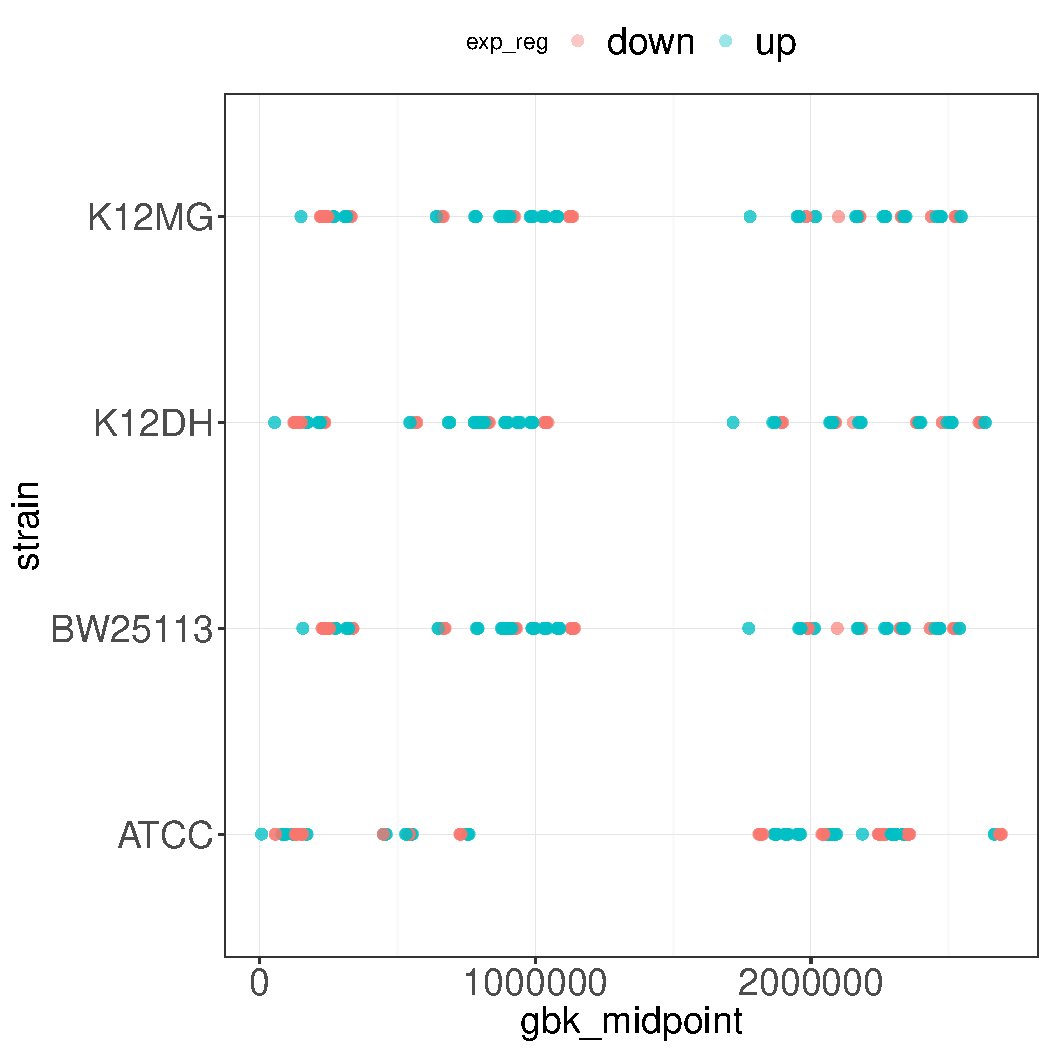
\includegraphics[width=\textwidth]{genome_pos_inversions_attempt1.pdf}
		\caption{\label{fig:inversions_pos_1} An attempt at showing all taxa and the significant inversions (significant $=$ blocks that had a significant difference in gene expression between inverted and non-inverted sequences using wilcox sign-ranked test). The ``up'' and ``down'' simply mean that the sequences that were inverted in that block has significantly higher or lower gene expression than the non-inverted sequences in that block. This up/down was NOT done using DESeq, just a simple wilcox sign-ranked test.}
	\end{center}
\end{figure}

\begin{figure}[h]
	\begin{center}
		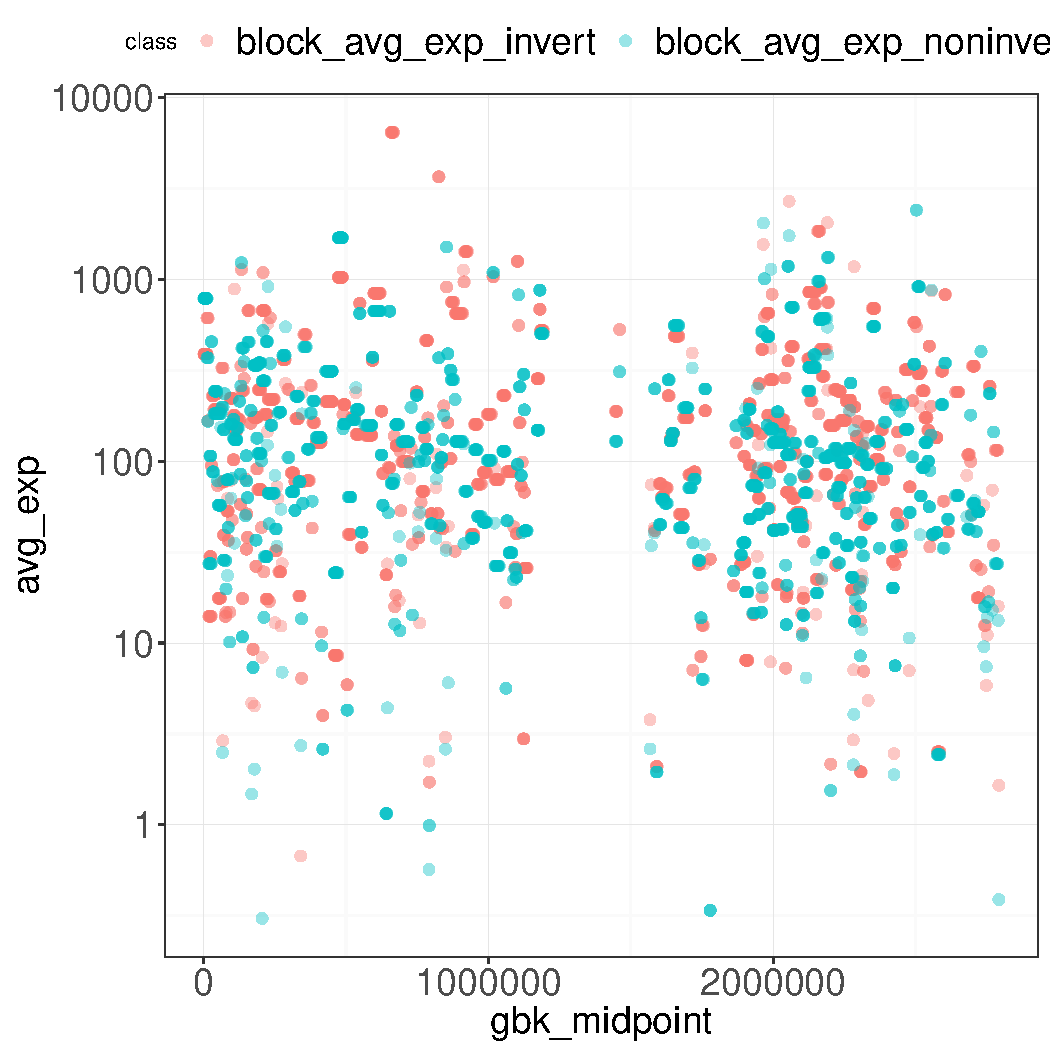
\includegraphics[width=\textwidth]{genome_pos_inversions_k12.pdf}
		\caption{\label{fig:inversions_pos_2} An attempt at showing just the significant inversions (significant $=$ blocks that had a significant difference in gene expression between inverted and non-inverted sequences using wilcox sign-ranked test) using the distance from the origin of \ecol K12 MG655. The ``up'' and ``down'' simply mean that the sequences that were inverted in that block has significantly higher or lower gene expression than the non-inverted sequences in that block. This up/down was NOT done using DESeq, just a simple wilcox sign-ranked test.}
	\end{center}
\end{figure}

\begin{figure}[h]
	\begin{center}
		\includegraphics[width=\textwidth]{genome_pos_inversions_sketch.png}
		\caption{\label{fig:inversions_pos_sketch} A sketch of what I am hoping the position graph would look like. Each inverted region/block would be plotted and the average gene expression of the inverted and non-inverted sequences would be in different colours (green and yellow). Any blocks that had a significant difference in gene expression (significant $=$ blocks that had a significant difference in gene expression between inverted and non-inverted sequences using wilcox sign-ranked test), would be somehow bold in the diagram (red box).}
	\end{center}
\end{figure}

\end{document}
